\documentclass[10pt, aspectratio=149]{beamer}

% Include preamble files
\input{preamble/packages}
\input{preamble/commands}
\input{preamble/beamer_settings}

\title[Generative Adversarial Networks (GANs)]{Generative Adversarial Networks (GANs)}

\begin{document}

% Include sections
\input{sections/cover-KA+LMH}
% \begin{frame}[plain]
    \begin{figure}
        \centering
        \fetchconvertimage{https://miro.medium.com/v2/resize:fit:1115/1*cpIITkxg8Ven2ohs5PqsTg.png}{images/vector-space/cover.png}{width=\textwidth,height=0.9\textheight,keepaspectratio}
    \end{figure}
\end{frame}

% Table of Contents
\begin{frame}[allowframebreaks]{Table of Contents}
\begin{enumerate}
    \item Objectives
    \item Motivation
    \item Summary
\end{enumerate}
\end{frame}
\section{Motivation}

\begin{frame}[t]{Welcome to CNNs!}
    \textbf{Topic: Introduction to Convolution and CNNs}

    \vspace{1em}
    \textbf{What we’ll learn today:}
    \begin{itemize}
        \item How computers see images
        \item What is convolution
        \item How CNNs work
        \item Implementing CNNs in PyTorch
    \end{itemize}
\end{frame}

\begin{frame}[allowframebreaks]{Motivation}
    \begin{figure}
        \centering
        \includegraphics[height=0.9\textheight,width=1\textwidth,keepaspectratio]{images/cnn/represent_image.png}
    \end{figure}

    \begin{itemize}
        \item Humans are amazing at understanding images: recognizing faces, reading signs, identifying objects.
        \item Computers? Not so much. They need help!
    \end{itemize}

    \framebreak

    \begin{figure}
        \centering
        \includegraphics[height=0.8\textheight,width=0.8\textwidth,keepaspectratio]{images/cnn/represent_image.png}
    \end{figure}

    \begin{itemize}
        \item What we human see as a simple image is just a grid (or matrix) of numbers to a computer.
        \item Each pixel has a value (0-255 for grayscale, 3 values for RGB).
        \item Computers need to learn patterns in these numbers to understand images.
        \framebreak
        \item \large Convolution and CNNs are the backbone of modern computer vision.
        \item Used in self-driving cars, medical diagnosis, facial recognition, etc.
    \end{itemize}
\end{frame}

\begin{frame}[allowframebreaks]{Some Applications}

    \foreach \i in {2,...,13} { % Integers from 1 to 5
        \begin{figure}
            \centering
            \includegraphics[height=0.9\textheight,width=1\textwidth,keepaspectratio]{images/cnn/cv_\i.png}
        \end{figure}

        \framebreak
    }

    % \begin{figure}
    %     \centering
    %     \includegraphics[height=0.9\textheight,width=1\textwidth,keepaspectratio]{images/cnn/cv_2.png}
    % \end{figure}

    % \framebreak

    % \begin{figure}
    %     \centering
    %     \includegraphics[height=0.9\textheight,width=1\textwidth,keepaspectratio]{images/cnn/cv_3.png}
    % \end{figure}

    % \framebreak

    % \begin{figure}
    %     \centering
    %     \includegraphics[height=0.8\textheight,width=1\textwidth,keepaspectratio]{images/cnn/cv_4.png}
    % \end{figure}

    % \framebreak

    % \begin{figure}
    %     \centering
    %     \includegraphics[height=0.8\textheight,width=1\textwidth,keepaspectratio]{images/cnn/cv_5.png}
    % \end{figure}

    % \framebreak
\end{frame}

\begin{frame}[allowframebreaks]{Motivation}
    \begin{itemize}
        \item \textbf{Transformative Impact:} Convolutional Neural Networks (CNNs) have revolutionized computer vision and deep learning.
        \item \textbf{Wide Applications:} Power tasks such as image classification, object detection, facial recognition, and medical image analysis.
        \item \textbf{Automatic Feature Learning:} CNNs learn hierarchical features directly from raw pixel data, reducing the need for manual feature engineering.
        \item \textbf{Demystifying CNNs:} This presentation breaks down core components and traces the evolution of key architectures.
        \item \textbf{Practical Relevance:} Understanding CNNs enables better design, optimization, and application to real-world problems.
    \end{itemize}
\end{frame}
\section{Objectives \& Learning Outcomes}
\begin{frame}{}
    \LARGE GANs: \textbf{Objectives \& Learning Outcomes}
\end{frame}

\begin{frame}[allowframebreaks]{GANs: Objectives}
    \begin{enumerate}
        \setlength{\itemsep}{-0.1em}
        \item \textbf{Understand the fundamental concepts and motivations behind GANs.}
        \begin{enumerate}
            \setlength{\itemsep}{-0.75em}
            \item Learn why GANs were introduced and what problems they aim to solve in generative modeling.
        \end{enumerate}
        \item \textbf{Explore the mathematical formulation and training process of GANs.}
        \begin{enumerate}
            \setlength{\itemsep}{-0.75em}
            \item Study the minimax objective and the roles of the generator and discriminator.
            \item Analyze how GANs compare distributions via samples.
        \end{enumerate}
        \item \textbf{Examine objective functions and training challenges.}
        \begin{enumerate}
            \setlength{\itemsep}{-0.75em}
            \item Review standard and alternative objective functions.
            \item Identify common problems in GAN training, such as mode collapse and instability.
        \end{enumerate}
        \item \textbf{Survey popular GAN variants and latent space concepts.}
        \begin{enumerate}
            \setlength{\itemsep}{-0.75em}
            \item Wasserstein GANs, Conditional GANs, CycleGANs, StyleGANs.
            \item Understand the role and selection of latent spaces in GANs.
        \end{enumerate}
    \end{enumerate}
\end{frame}

\begin{frame}[allowframebreaks]{\textcolor{green}{$\Rightarrow$} Learning Outcomes}
    By the end of this session, you will be able to:
    \begin{enumerate}
        \item Understand how GANs work at a high level.
        \item Describe the roles of the Generator and Discriminator.
        \item Explain how GANs are trained.
        \item Recognize major variants of GANs.
        \item Understand challenges and limitations of GANs.
    \end{enumerate}
\end{frame}
\section{Introduction}
\begin{frame}{}
    \LARGE GANs: \textbf{Introduction}
\end{frame}

\begin{frame}[allowframebreaks]{Comparing Distributions via Samples}
Given a finite set of samples from two distributions $S_1 = \{x \sim P\}$ and $S_2 = \{x \sim Q\}$, how can we tell if these samples are from the same distribution? (i.e., $P = Q$?)
\begin{figure}
    \centering
    \includegraphics[height=0.58\textheight, width=\textwidth, keepaspectratio]{images/gan/gan_two_dist.png}
\end{figure}

% Place this at the bottom of the frame, before \end{frame}
% \vspace{0.5em}
\begin{minipage}{\textwidth}
\footnotetext{GANs aim to replicate data distributions, but we rarely have access to
the true probability distribution function. Instead, we compare samples
from the real data distribution with those generated by the model.}
\end{minipage}

\framebreak

\begin{itemize}
    \item Let's consider a test statistic $T$ for this purpose.
    \item Test statistic $T$ compares $S_1$ and $S_2$ e.g., difference in means, variances of the two sets of samples.
    \item \textbf{Key observation}: Test statistic is likelihood-free since it does not involve the densities $P$ or $Q$ (only samples)
\end{itemize}
\end{frame}
\begin{frame}{What is Deep Unsupervised Learning?}
    \textbf{Deep Unsupervised Learning} aims to discover \textbf{hidden patterns} and \textbf{structures} in raw data using deep neural networks, \textbf{without any human-provided labels}. 
    
    It focuses on \textbf{capturing rich patterns in raw data with deep networks in a label-free way}.
        \begin{itemize}
            \item \textbf{Learns from observation} --- mimics how humans learn from experience
            \item \textbf{Discovers structure} --- finds groups, similarities, and representations
            \item \textbf{Scales to complex data} --- uses deep models to capture abstract features
            \item \textbf{Generative Models} --- recreate raw data distribution
            \item \textbf{Self-supervised Learning} --- “puzzle” tasks that require semantic understanding
        \end{itemize}
        \vspace{0.5em}
        \centering
        {\Large \textbf{Why do we care?}}
\end{frame}

\begin{frame}{}
    \begin{center}
    \begin{minipage}{0.9\textwidth}
        \begin{columns}
            \column{0.2\textwidth}
                \includegraphics[width=0.8\linewidth]{images/dul/slide_15_1_img.png}
            \column{0.5\textwidth}
                \centering
                \textbf{Geoffrey Hinton}\\
                (in his 2014 AMA on Reddit)
        \end{columns}
        \vspace{1em}
        \begin{center}
        \textit{“The brain has about $10^{14}$ synapses and we only live for about $10^{9}$ seconds. 
        So we have a lot more parameters than data. This motivates the idea that we must do a lot of 
        unsupervised learning since the perceptual input (including proprioception) is the only place 
        we can get $10^{5}$ dimensions of constraint per second.”}
        \end{center}
    \end{minipage}
    \end{center}
\end{frame}

\begin{frame}{}
    \begin{columns}
        \column{0.3\textwidth}
            \centering
            \includegraphics[width=0.8\linewidth]{images/dul/slide_16_2_img.png}
            \textbf{Yann LeCun}\\[1em]
            \textcolor{blue}{Need tremendous amount of information to build machines that have common sense and generalize well.}\\[1em]
            [LeCun-20161205-NeurIPS-keynote]
        \column{0.7\textwidth}
            \includegraphics[width=1.05\linewidth]{images/dul/slide_16_1_img.png}
    \end{columns}
\end{frame}

\begin{frame}{``Ideal Intelligence``}
    \begin{itemize}
        \item \textbf{“Ideal Intelligence” is all about compression} (finding all patterns)
        \item Finding all patterns = short description of raw data (\textit{low Kolmogorov Complexity})
        \item Shortest code-length = optimal inference (\textit{Solomonoff Induction})
        \item Extensible to optimal action-making agents (\textit{AIXI})
    \end{itemize}
    \vspace{1em}
    \textbf{Transfer Learning via Compression:}
    \begin{itemize}
        \item Assume we pretrain unsupervised on Data Distribution $D_1$ and then finetune on Data Distribution $D_2$
        \item If $D_1$ and $D_2$ are related, compressing $D_2$ conditioned on $D_1$ should be more efficient than compressing $D_2$ outright
        \item \textbf{Hence:} pretraining on $D_1$ should aid faster learning of $D_2$
    \end{itemize}
\end{frame}
\section{Training}
\begin{frame}{}
    \LARGE GANs: \textbf{Training}
\end{frame}

\begin{frame}[allowframebreaks]{Training}
\begin{itemize}
    \item Both Discriminator and Generator are trained jointly in a min-max game.
    \item Minimax objective function:
    $$\min_{\theta_G} \max_{\theta_D} = E_{x \sim p_{data}} log(\underbrace{D_{\theta_D}(x)}_{\substack{\text{Discriminator}\\ \text{output for}\\ \text{real data }x}}) + E_{x \sim p(z)} log(1-\underbrace{D_{\theta_D}(G_{\theta_G}(z))}_{\substack{\text{Discriminator output}\\ \text{for generated fake}\\ \text{data } G(z)}})$$
    \item Discriminator $\theta_D$ wants to maximise objective such that $D(x)$ is close to 1 (real) and $D(G(z))$ is close to 0 (fake).
    \item Generator $\theta_G$ wants to minimise objective such that $D(G(z))$ is close to 1 (discriminator is fooled into thinking generated $G(z)$ is real).

\end{itemize}

\framebreak
\begin{figure}
    \centering
    \includegraphics[height=1\textheight, width=1.02\textwidth, keepaspectratio]{images/gan/pseudocode.png}
\end{figure}

\framebreak
\textbf{The Adversarial Process:}
\begin{enumerate}
    \item Discriminator is trained to distinguish real from fake.
    \item Generator is trained to fool the discriminator.
    \item Repeat: Alternate steps until convergence.
\end{enumerate}

\textbf{Training Tips:}
\begin{itemize}
    \item Use batch normalization.
    \item Avoid sigmoid output in discriminator.
    \item Use Leaky ReLU in discriminator.
\end{itemize}

\textbf{Practical Issues:}
\begin{itemize}
    \item Discriminator becomes too strong.
    \item Gradient vanishing for generator.
    \item Careful balance of training speeds is necessary.
\end{itemize}
    
\end{frame}
\section{Objective function}
\begin{frame}{}
    \LARGE GANs: \textbf{Objective function}
\end{frame}

\begin{frame}[allowframebreaks]{Understanding the Objective function}
The goal of GANs is to find a \textbf{Nash equilibrium} between the generator and discriminator. 
The generator tries to minimize the probability of the discriminator correctly classifying fake data.
\begin{figure}
    \centering
    \includegraphics[height=0.7\textheight, width=\textwidth, keepaspectratio]{images/gan/gan_cost_1.png}
\end{figure}

\framebreak
\begin{figure}
    \centering
    \includegraphics[height=0.9\textheight, width=\textwidth, keepaspectratio]{images/gan/gan_cost_2.png}
\end{figure}

\framebreak
\begin{figure}
    \centering
    \includegraphics[height=0.9\textheight, width=\textwidth, keepaspectratio]{images/gan/gan_cost_3.png}
\end{figure}

\framebreak
\begin{figure}
    \centering
    \includegraphics[height=0.9\textheight, width=\textwidth, keepaspectratio]{images/gan/gan_cost_4.png}
\end{figure}

\framebreak
\begin{figure}
    \centering
    \includegraphics[height=0.9\textheight, width=\textwidth, keepaspectratio]{images/gan/gan_cost_5.png}
\end{figure}


\footnotetext{https://www.slideshare.net/ckmarkohchang/generative-adversarial-networks}
\end{frame}

\begin{frame}{GANs - Interactive Demo}
\centering
\href{https://poloclub.github.io/ganlab/}{https://poloclub.github.io/ganlab/}
    
\end{frame}
\section{Results}
\begin{frame}{}
    \LARGE GANs: \textbf{Results}
\end{frame}

\begin{frame}[allowframebreaks]{Results}
\begin{figure}
    \centering
    \includegraphics[height=0.8\textheight, width=\textwidth, keepaspectratio]{images/gan/result-goodfellow.png}
    \caption*{Figure from Goodfellow et al 2014, showing GAN results on various datasets.}
\end{figure}

\framebreak
\begin{figure}
    \centering
    \includegraphics[height=0.8\textheight, width=\textwidth, keepaspectratio]{images/gan/gan_results_mnist.png}
    \caption*{GAN generated samples for MNIST digits dataset}
\end{figure}

\framebreak
\begin{figure}
    \centering
    \includegraphics[height=0.8\textheight, width=\textwidth, keepaspectratio]{images/gan/gan_results_2.png}
    \caption*{GAN generated samples for bedroom images}
\end{figure}

\framebreak
\begin{figure}
    \centering
    \includegraphics[height=0.8\textheight, width=\textwidth, keepaspectratio]{images/gan/gan_results_3.png}
    \caption*{GAN generated samples for anime character faces}
\end{figure}
    
\end{frame}
\section{Problems}
\begin{frame}{}
    \LARGE GANs: \textbf{Problems}
\end{frame}

\begin{frame}[allowframebreaks]{Problems with GANs}
\textbf{\large Vanishing Gradients }
    \begin{itemize}
        \item When the discriminator is perfect, we are guaranteed with $D(x) = 1, \forall x \in p_{data}$ and $D(x) = 0, \forall x \in p_G$.
        \item The loss function drops to zero, resulting in no gradient for updates.
        \item \textbf{Solution}: Perform gradient ascent on the generator, i.e., use a different objective:
        $$\max_{\theta_G} E_{x \sim p(z)} log(D_{\theta_D}(G_{\theta_G}(z)))$$
    \end{itemize}
\framebreak

\begin{figure}
    \centering
    \includegraphics[height=0.8\textheight, width=\textwidth, keepaspectratio]{images/gan/gan_generator_gradient.png}
    \caption*{Vanishing gradient in GANs (Image source: \href{https://arxiv.org/pdf/1701.04862.pdf}{Arjovsky and Bottou, 2017})}
\end{figure}

\framebreak

\textbf{\large Difficulty in achieving Nash equilibrium}
    \begin{itemize}
        \item GANs involve training two models simultaneously to reach a Nash equilibrium in a two-player non-cooperative game. However, since each model updates its cost independently, convergence is not guaranteed.
        \item For practical tips on training GANs, see "How to Train a GAN? Tips and tricks to make GANs work" by Soumith Chintala: \href{https://github.com/soumith/ganhacks}{https://github.com/soumith/ganhacks}
    \end{itemize}

\framebreak
\textbf{\large Mode collapse}
    \begin{itemize}
        \item The generator aims to fool the discriminator $D$ into classifying its outputs as real. If the generator $G$ finds a single output that consistently fools $D$, it may repeatedly produce that output, leading to mode collapse.
        \item Solutions to mode collapse are mostly empirical, including alternative architectures, modified GAN losses, and additional regularization terms.
        
        \begin{figure}
            \centering
            \includegraphics[height=0.4\textheight, width=\textwidth, keepaspectratio]{images/gan/gan_mode_collapse_1.png}
        \end{figure}
    \end{itemize}

\framebreak
\begin{figure}
    \centering
    \includegraphics[height=0.85\textheight, width=\textwidth, keepaspectratio]{images/gan/gan_mode_collapse_2.png}
    \caption*{GAN mode collapse on MNIST digits dataset}
\end{figure}
    
\end{frame}
\begin{frame}{}
    \LARGE GANs: \textbf{Variants}
\end{frame}

\begin{frame}[allowframebreaks]{GAN Variants}
\begin{itemize}
    \item Since the introduction of GANs, extensive research has led to many variants.
    \item A comprehensive list of GAN variants can be found \href{https://github.com/hindupuravinash/the-gan-zoo}{here}.
\end{itemize} 
    \framebreak
    
    We will discuss the following variants:
    \begin{itemize}
        \item \textbf{Deep Convolutional GAN (DCGAN):}
        \begin{itemize}
            \item Uses convolutional and transposed convolutional layers.
            \item Employs batch normalization and ReLU/LeakyReLU activations.
            \item Improves training stability and image quality.
        \end{itemize}
        \item \textbf{Wasserstein GAN (WGAN):} 
        \begin{itemize}
            \item Introduces Wasserstein distance as the objective.
            \item Replaces sigmoid with linear output.
            \item Uses weight clipping or gradient penalty.
            \item \textbf{Variants:}
            \begin{itemize}
                \item \textbf{WGAN-GP:} Uses gradient penalty instead of weight clipping for better stability.
                \item \textbf{WGAN-LP:} Uses Lipschitz penalty as an alternative to gradient penalty.
            \end{itemize}
        \end{itemize}

\framebreak

        \item \textbf{Conditional GAN (cGAN):} 
        \begin{itemize}
            \item Conditions both the generator and discriminator on additional information (e.g., class labels).
            \item Useful for targeted generation.
        \end{itemize}
        \item \textbf{CycleGAN:} 
        \begin{itemize}
            \item Enables unpaired image-to-image translation.
            \item Uses cycle consistency loss to ensure invertibility.
        \end{itemize}
        \item \textbf{StyleGAN:} 
        \begin{itemize}
            \item Developed by NVIDIA for high-fidelity face generation.
            \item Introduces style vectors at each generator layer.
            \item Allows fine-grained control over image features.
        \end{itemize}
    \end{itemize}
\end{frame}

\subsection{Deep Convolutional GAN (DCGAN)}
\begin{frame}{}
    \LARGE GAN Variant: \\[1.5ex] \textbf{Deep Convolutional GAN (DCGAN)}
\end{frame}

\begin{frame}[allowframebreaks]{DCGAN}
    \begin{figure}
        \centering
        \includegraphics[height=0.9\textheight,keepaspectratio]{images/gan/dcgan-paper.png}
    \end{figure}

    \framebreak

    \begin{figure}
        \centering
        \includegraphics[width=1.05\textwidth,keepaspectratio]{images/gan/dcgan-architecture.png}
        \small [Radford et al 2016]
    \end{figure}

    \framebreak

    \textbf{Architecture Design Principles:}
    \begin{itemize}
        \item Utilizes convolutional and transposed convolutional layers instead of fully connected layers.
        \item Key architectural guidelines:
            \begin{itemize}
                \item Standard supervised CNNs are not directly usable for GANs.
                \item Remove max-pooling and mean-pooling layers.
                \item Generator upsamples using transposed convolutions.
                \item Discriminator downsamples with strided convolutions and average pooling.
                \item Non-linearity: ReLU for generator (except output), LeakyReLU (slope 0.2) for discriminator.
                \item Output non-linearity: \texttt{tanh} for generator, \texttt{sigmoid} for discriminator.
                \item Batch normalization is used to prevent mode collapse, but not applied at the output of G or input of D.
            \end{itemize}
        \item \textbf{Optimization}: Adam optimizer with learning rate $2 \times 10^{-4}$, momentum $0.5$, batch size $128$.
        \item Achieves stable training and generates high-quality images.
    \end{itemize}
\end{frame}
    
\begin{frame}[allowframebreaks]{DCGAN: Results}
    Good samples on datasets with 3M images (Faces, Bedrooms) for the first time
    \begin{figure}
        \centering
        \includegraphics[width=0.9\textwidth,keepaspectratio]{images/gan/dcgan-result-1.png}
    \end{figure}
    \footnotesize{Reference: Radford, Metz, and Chintala, "Unsupervised Representation Learning with Deep Convolutional Generative Adversarial Networks", ICLR 2016}

    \framebreak

    \begin{figure}
        \centering
        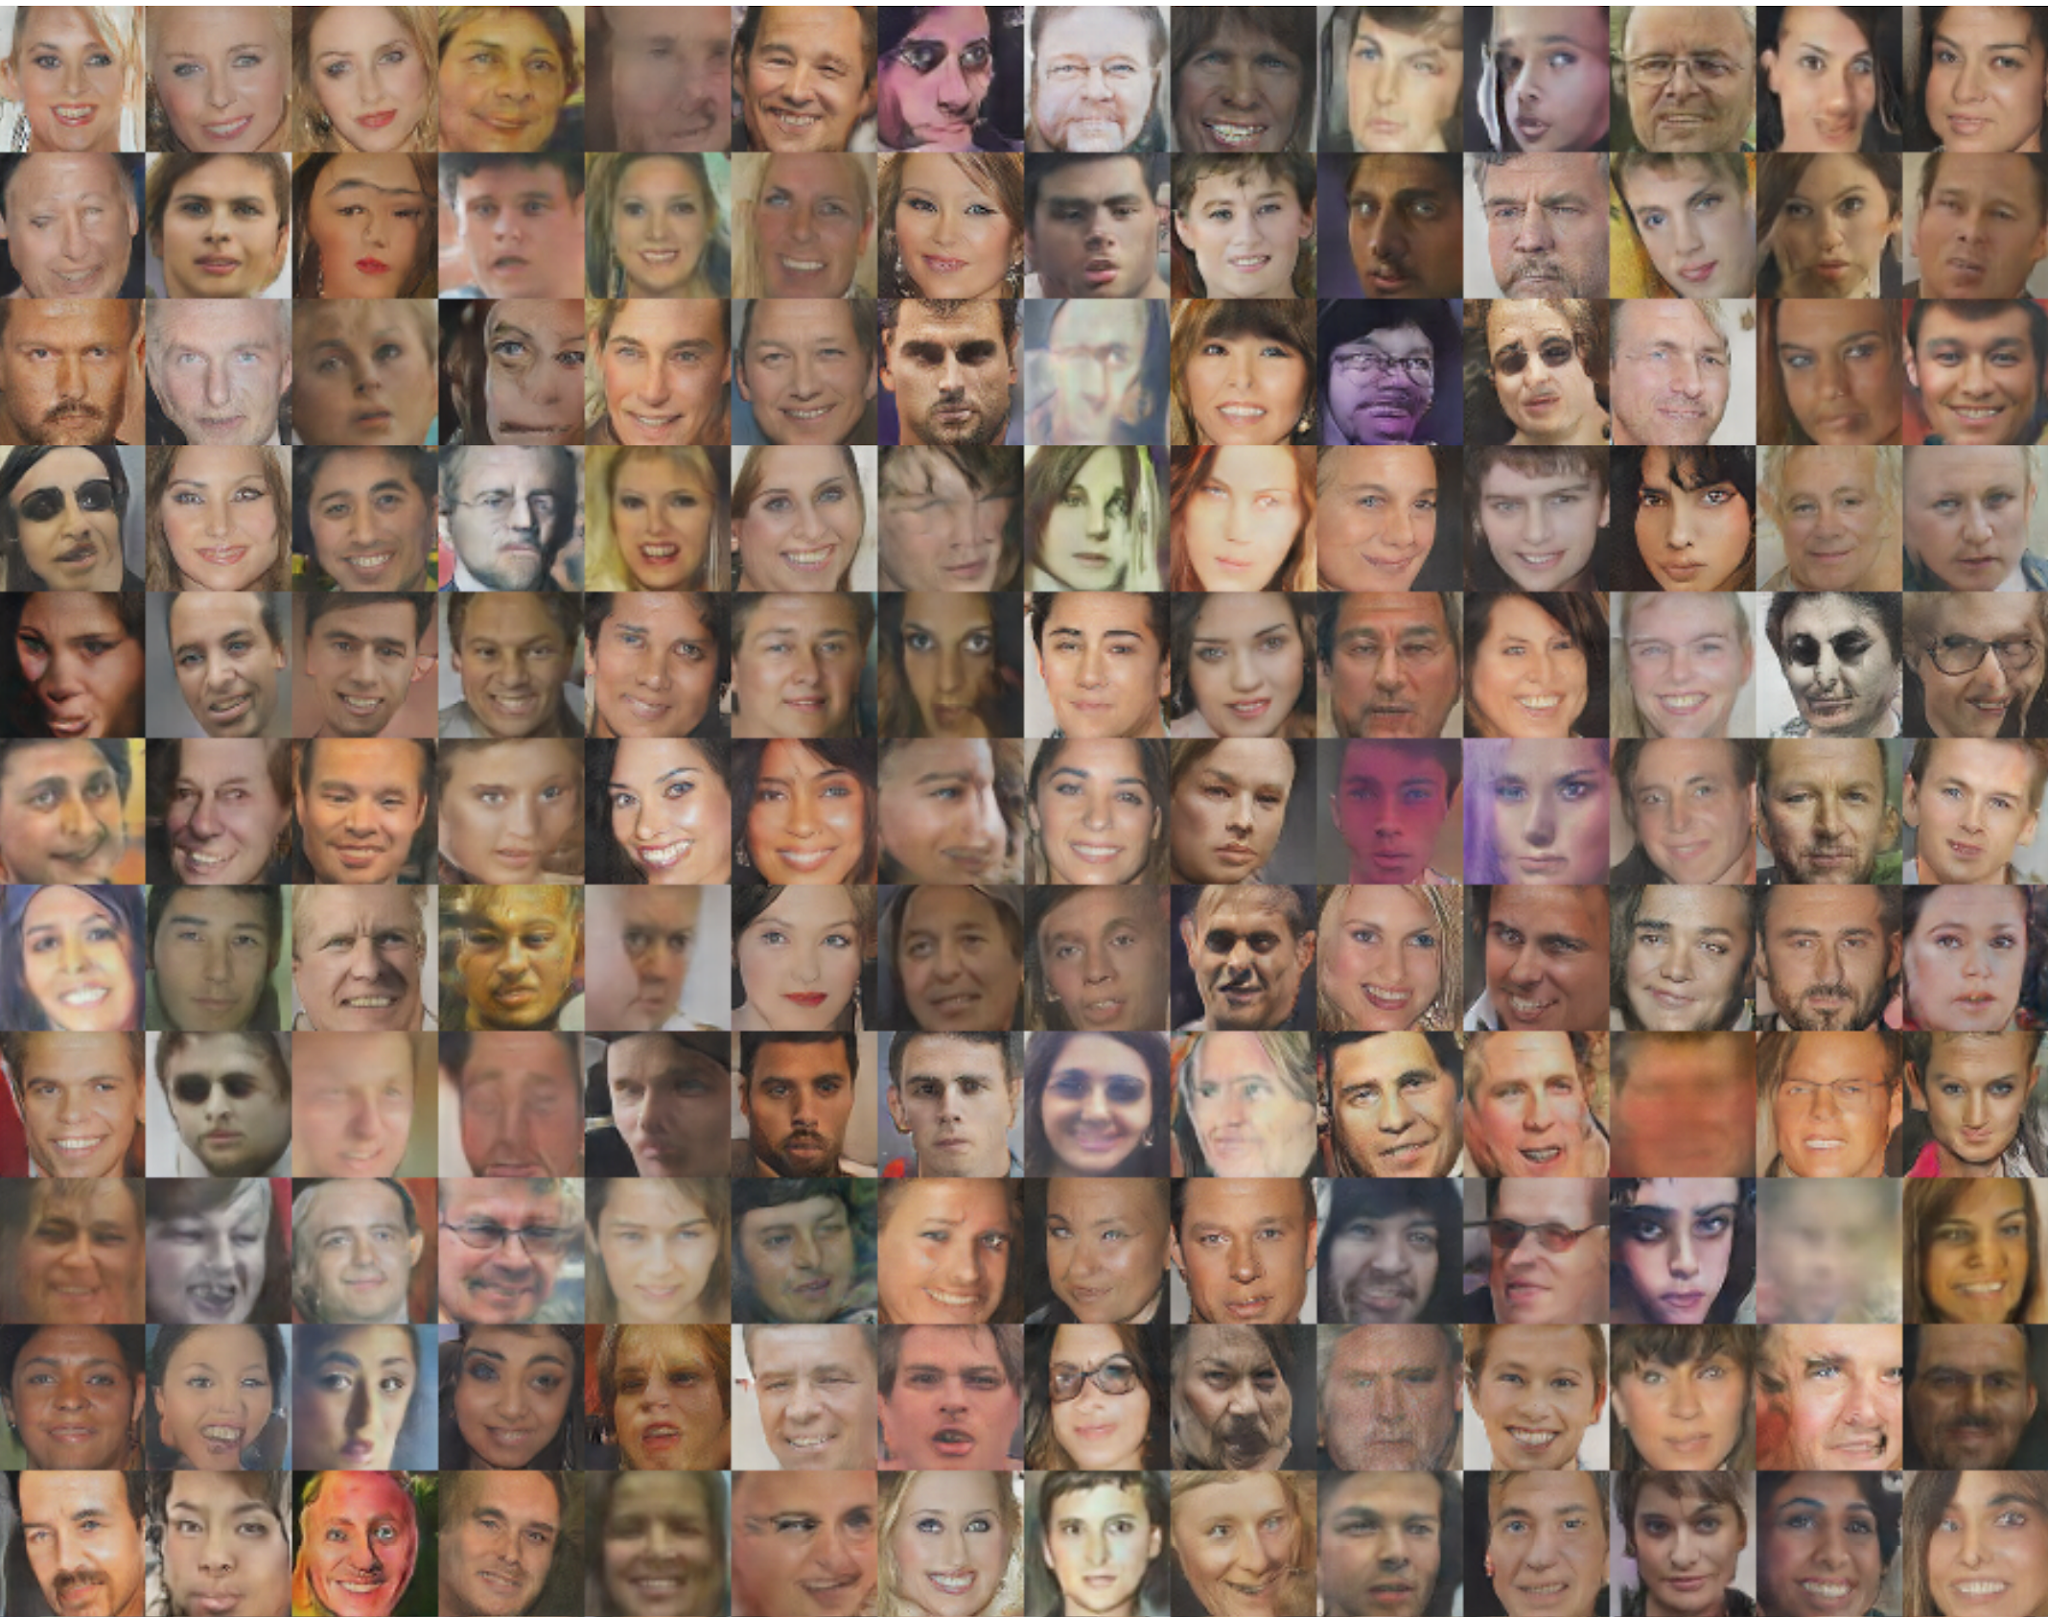
\includegraphics[height=0.8\textheight,keepaspectratio]{images/gan/dcgan-result-2.png}
        \caption*{[Radford et al 2016]} 
    \end{figure}

    \framebreak

    Smooth interpolations in high dimensions
    \begin{figure}
        \centering
        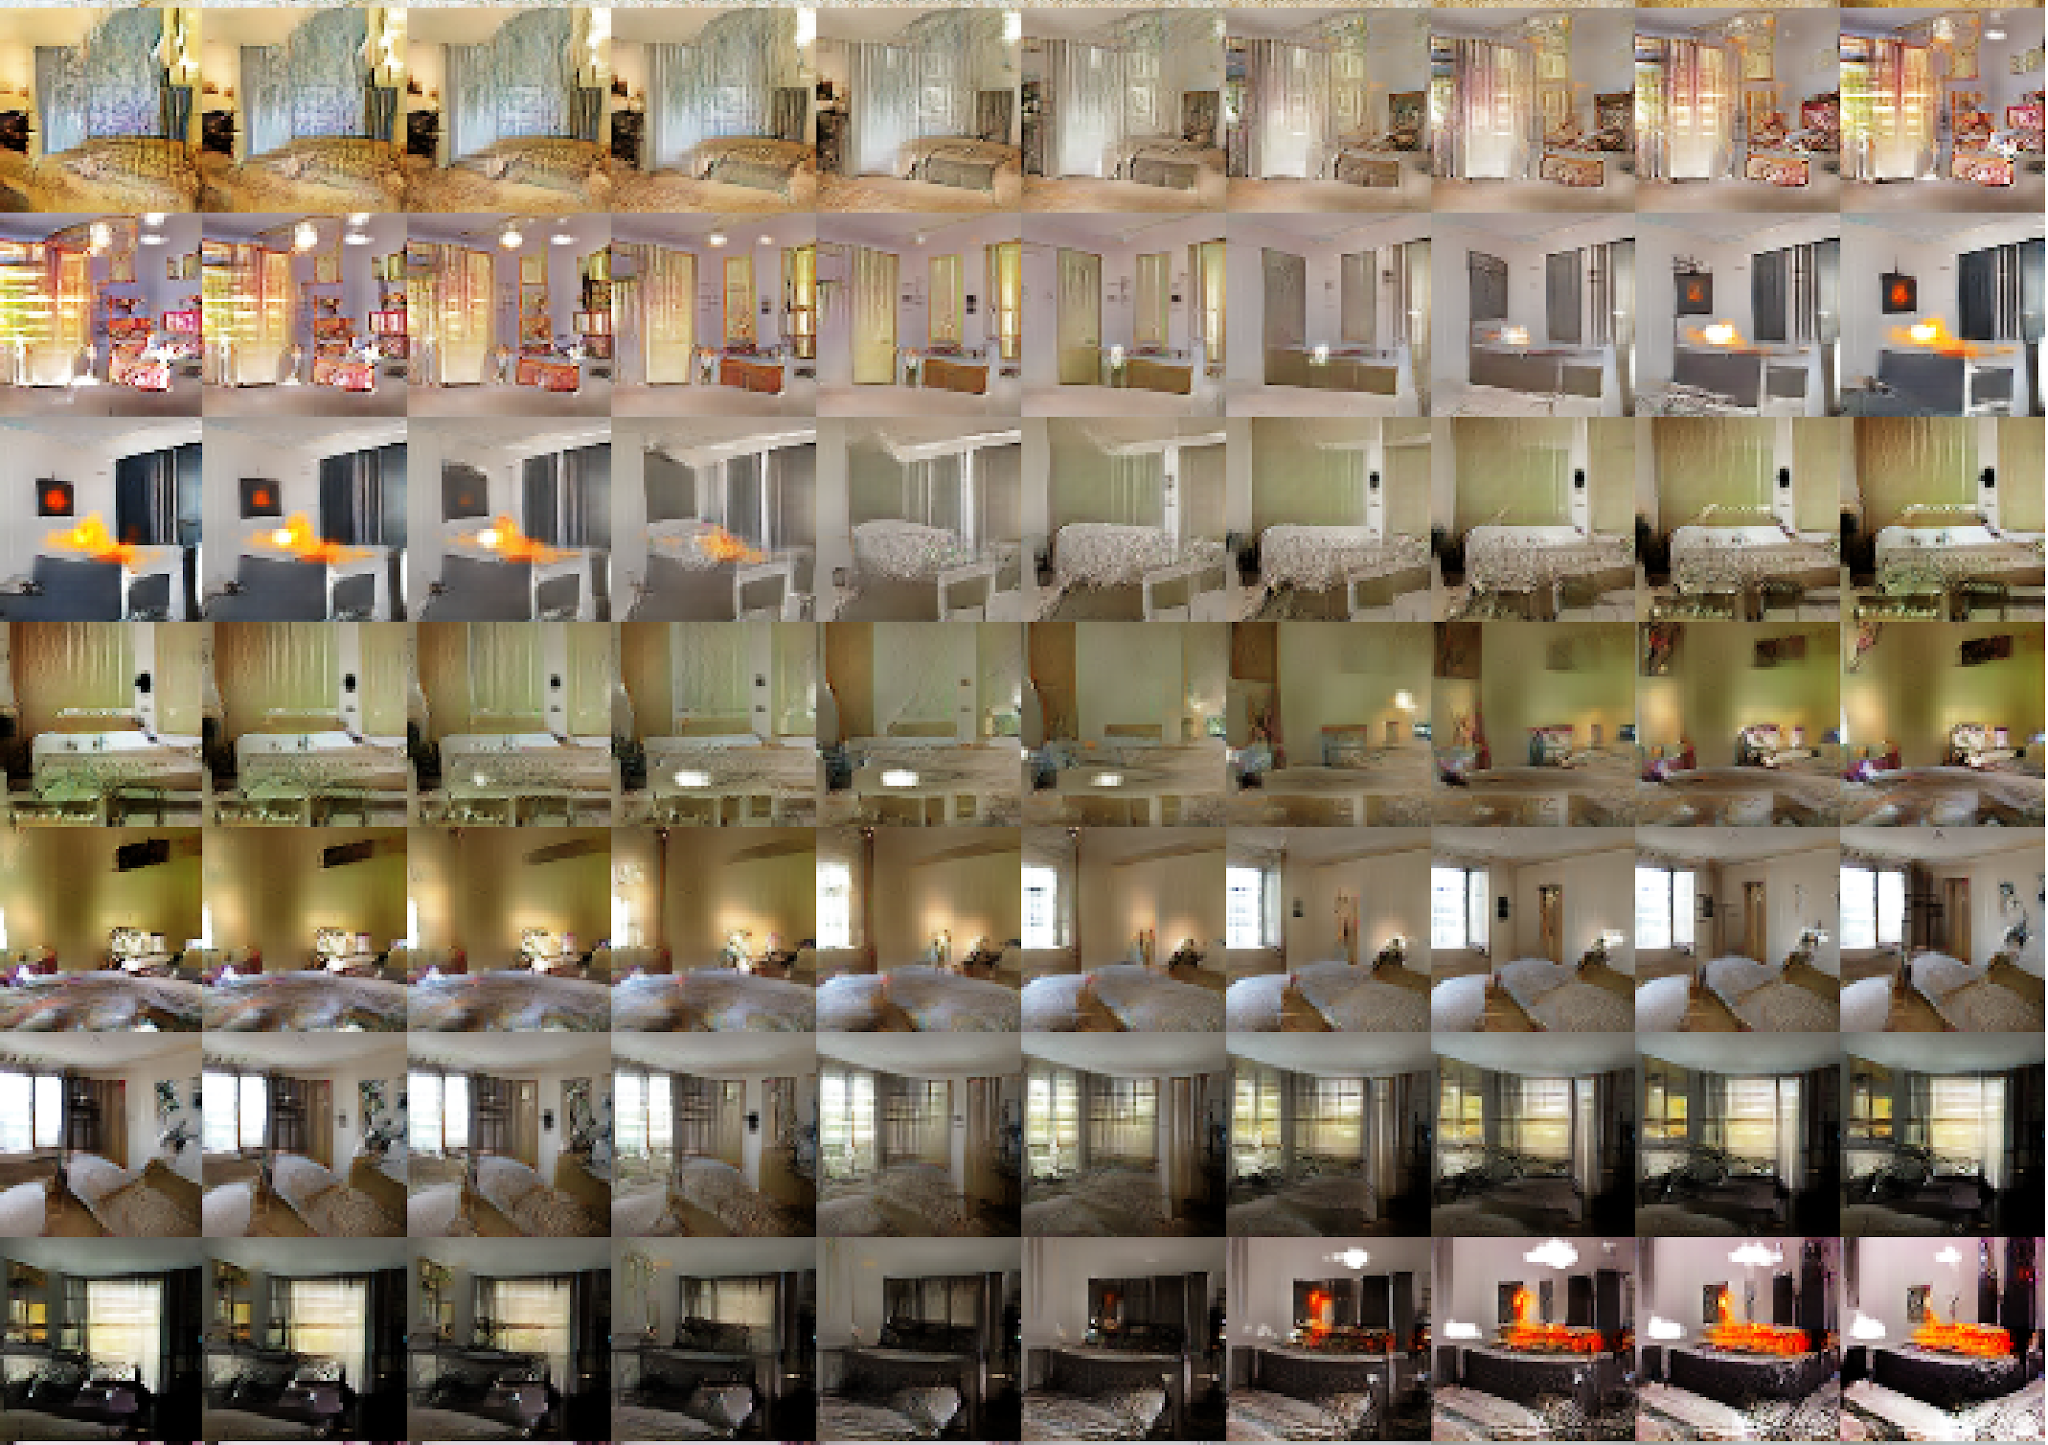
\includegraphics[height=0.8\textheight,keepaspectratio]{images/gan/dcgan-result-3.png}
        \caption*{[Radford et al 2016]}
    \end{figure}

    \framebreak

    Imagenet samples (32x32)
    \begin{figure}
        \centering
        \includegraphics[height=0.8\textheight,keepaspectratio]{images/gan/dcgan-result-4.png}
        \caption*{[Radford et al 2016]}
    \end{figure}

    \framebreak

    Vector Arithmetic
    \begin{figure}
        \centering
        \includegraphics[height=0.75\textheight,keepaspectratio]{images/gan/dcgan-result-5.png}
        \caption*{[Radford et al 2016]}
    \end{figure}

    \framebreak

    \begin{figure}
        \centering
        \includegraphics[height=0.8\textheight,keepaspectratio]{images/gan/dcgan-result-6.png}
        \caption*{[Radford et al 2016]}
    \end{figure}

    \framebreak

    \begin{figure}
        \centering
        \includegraphics[height=0.8\textheight,keepaspectratio]{images/gan/dcgan-result-7.png}
        \caption*{[Radford et al 2016]}
    \end{figure}

    \framebreak

    Representation Learning 
    \begin{figure}
        \centering
        \includegraphics[width=1.05\textwidth,keepaspectratio]{images/gan/dcgan-result-table.png}
        \caption*{[Radford et al 2016]}
    \end{figure}
\end{frame}
\subsection{Wasserstein GANs (WGANs)}
\begin{frame}{}
    \LARGE GAN Variant: \\[1.5ex] \textbf{Wasserstein GANs (WGANs)}
\end{frame}

\begin{frame}[allowframebreaks]{Wasserstein GAN}
\begin{itemize}
    \item Wasserstein GAN uses wasserstein distance instead of crossentropy loss.
    \item Wasserstein distance that has a smoother gradient everywhere.
        \begin{figure}
            \centering
            \includegraphics[height=0.6\textheight, width=\textwidth, keepaspectratio]{images/gan/wgan_1.png}
        \end{figure}
\end{itemize}
    
\end{frame}

\begin{frame}{Wasserstein Distance}
\begin{itemize}
    \item Intuitively, it is the shovels of earth moved to make two distributions look alike.
    \begin{figure}
        \centering
        \includegraphics[height=0.6\textheight, width=\textwidth, keepaspectratio]{images/gan/wgan_2.png}
        \caption*{Step by Step plan of moving dirt between piles $P$ and $Q$ to make them match}
    \end{figure}
    
\end{itemize}
    
\end{frame}

\begin{frame}[allowframebreaks]{WGAN}
\begin{figure}
    \centering
    \includegraphics[height=0.9\textheight, width=\textwidth, keepaspectratio]{images/gan/wgan_3.png}
\end{figure}

\framebreak
\begin{figure}
    \centering
    \includegraphics[height=0.9\textheight, width=\textwidth, keepaspectratio]{images/gan/wgan_4.png}
\end{figure}

\framebreak
\begin{figure}
    \centering
    \includegraphics[height=0.8\textheight, width=\textwidth, keepaspectratio]{images/gan/wgan_5.png}
    \caption*{WGAN generation results on bedroom images}
\end{figure}

\end{frame}

\begin{frame}[allowframebreaks]{WGAN-GP: Gradient Penalty for Lipschitzness}
\begin{figure}
    \centering
    \includegraphics[height=0.8\textheight, width=\textwidth, keepaspectratio]{images/gan/wgan-gp/slide_84_1_img.png}
    \caption*{[Gulrajani et al 2017]}
\end{figure}

\framebreak
\begin{columns}
    \column{0.6\textwidth}
    \begin{figure}
        \centering
        \includegraphics[height=0.8\textheight, width=\textwidth, keepaspectratio]{images/gan/wgan-gp/slide_85_3_img.png}
    \end{figure}
    \begin{figure}
        \centering
        \includegraphics[height=0.1\textheight, width=\textwidth, keepaspectratio]{images/gan/wgan-gp/slide_85_4_img.png}
    \end{figure}
    \column{0.5\textwidth}
    \begin{figure}
        \centering
        \includegraphics[height=0.8\textheight, width=1.05\textwidth, keepaspectratio]{images/gan/wgan-gp/slide_85_2_img.png}
    \end{figure}
    \begin{figure}
        \centering
        \includegraphics[height=0.8\textheight, width=1.05\textwidth, keepaspectratio]{images/gan/wgan-gp/slide_85_1_img.png}
    \end{figure}
\end{columns}
\end{frame}

\begin{frame}[allowframebreaks]{WGAN-GP: Pseudocode}
    \begin{figure}
        \centering
        \includegraphics[height=0.8\textheight, width=1.05\textwidth, keepaspectratio]{images/gan/wgan-gp/slide_86_1_img.png}
        \caption*{[Gulrajani et al 2017]}
    \end{figure}
\end{frame}

\begin{frame}[allowframebreaks]{WGAN-GP: BatchNorm}
    \begin{figure}
        \centering
        \includegraphics[height=0.8\textheight, width=1.05\textwidth, keepaspectratio]{images/gan/wgan-gp/slide_87_1_img.png}
        \caption*{[Gulrajani et al 2017]}
    \end{figure}
\end{frame}

\begin{frame}[allowframebreaks]{WGAN-GP: Robustness to architectures}
    \begin{figure}
        \centering
        \includegraphics[height=0.8\textheight, width=1.05\textwidth, keepaspectratio]{images/gan/wgan-gp/slide_88_1_img.png}
    \end{figure}
    \begin{figure}
        \centering
        \includegraphics[height=0.8\textheight, width=1.05\textwidth, keepaspectratio]{images/gan/wgan-gp/slide_88_2_img.png}
        \caption*{[Gulrajani et al 2017]}
    \end{figure}

    \framebreak

    \begin{figure}
        \centering
        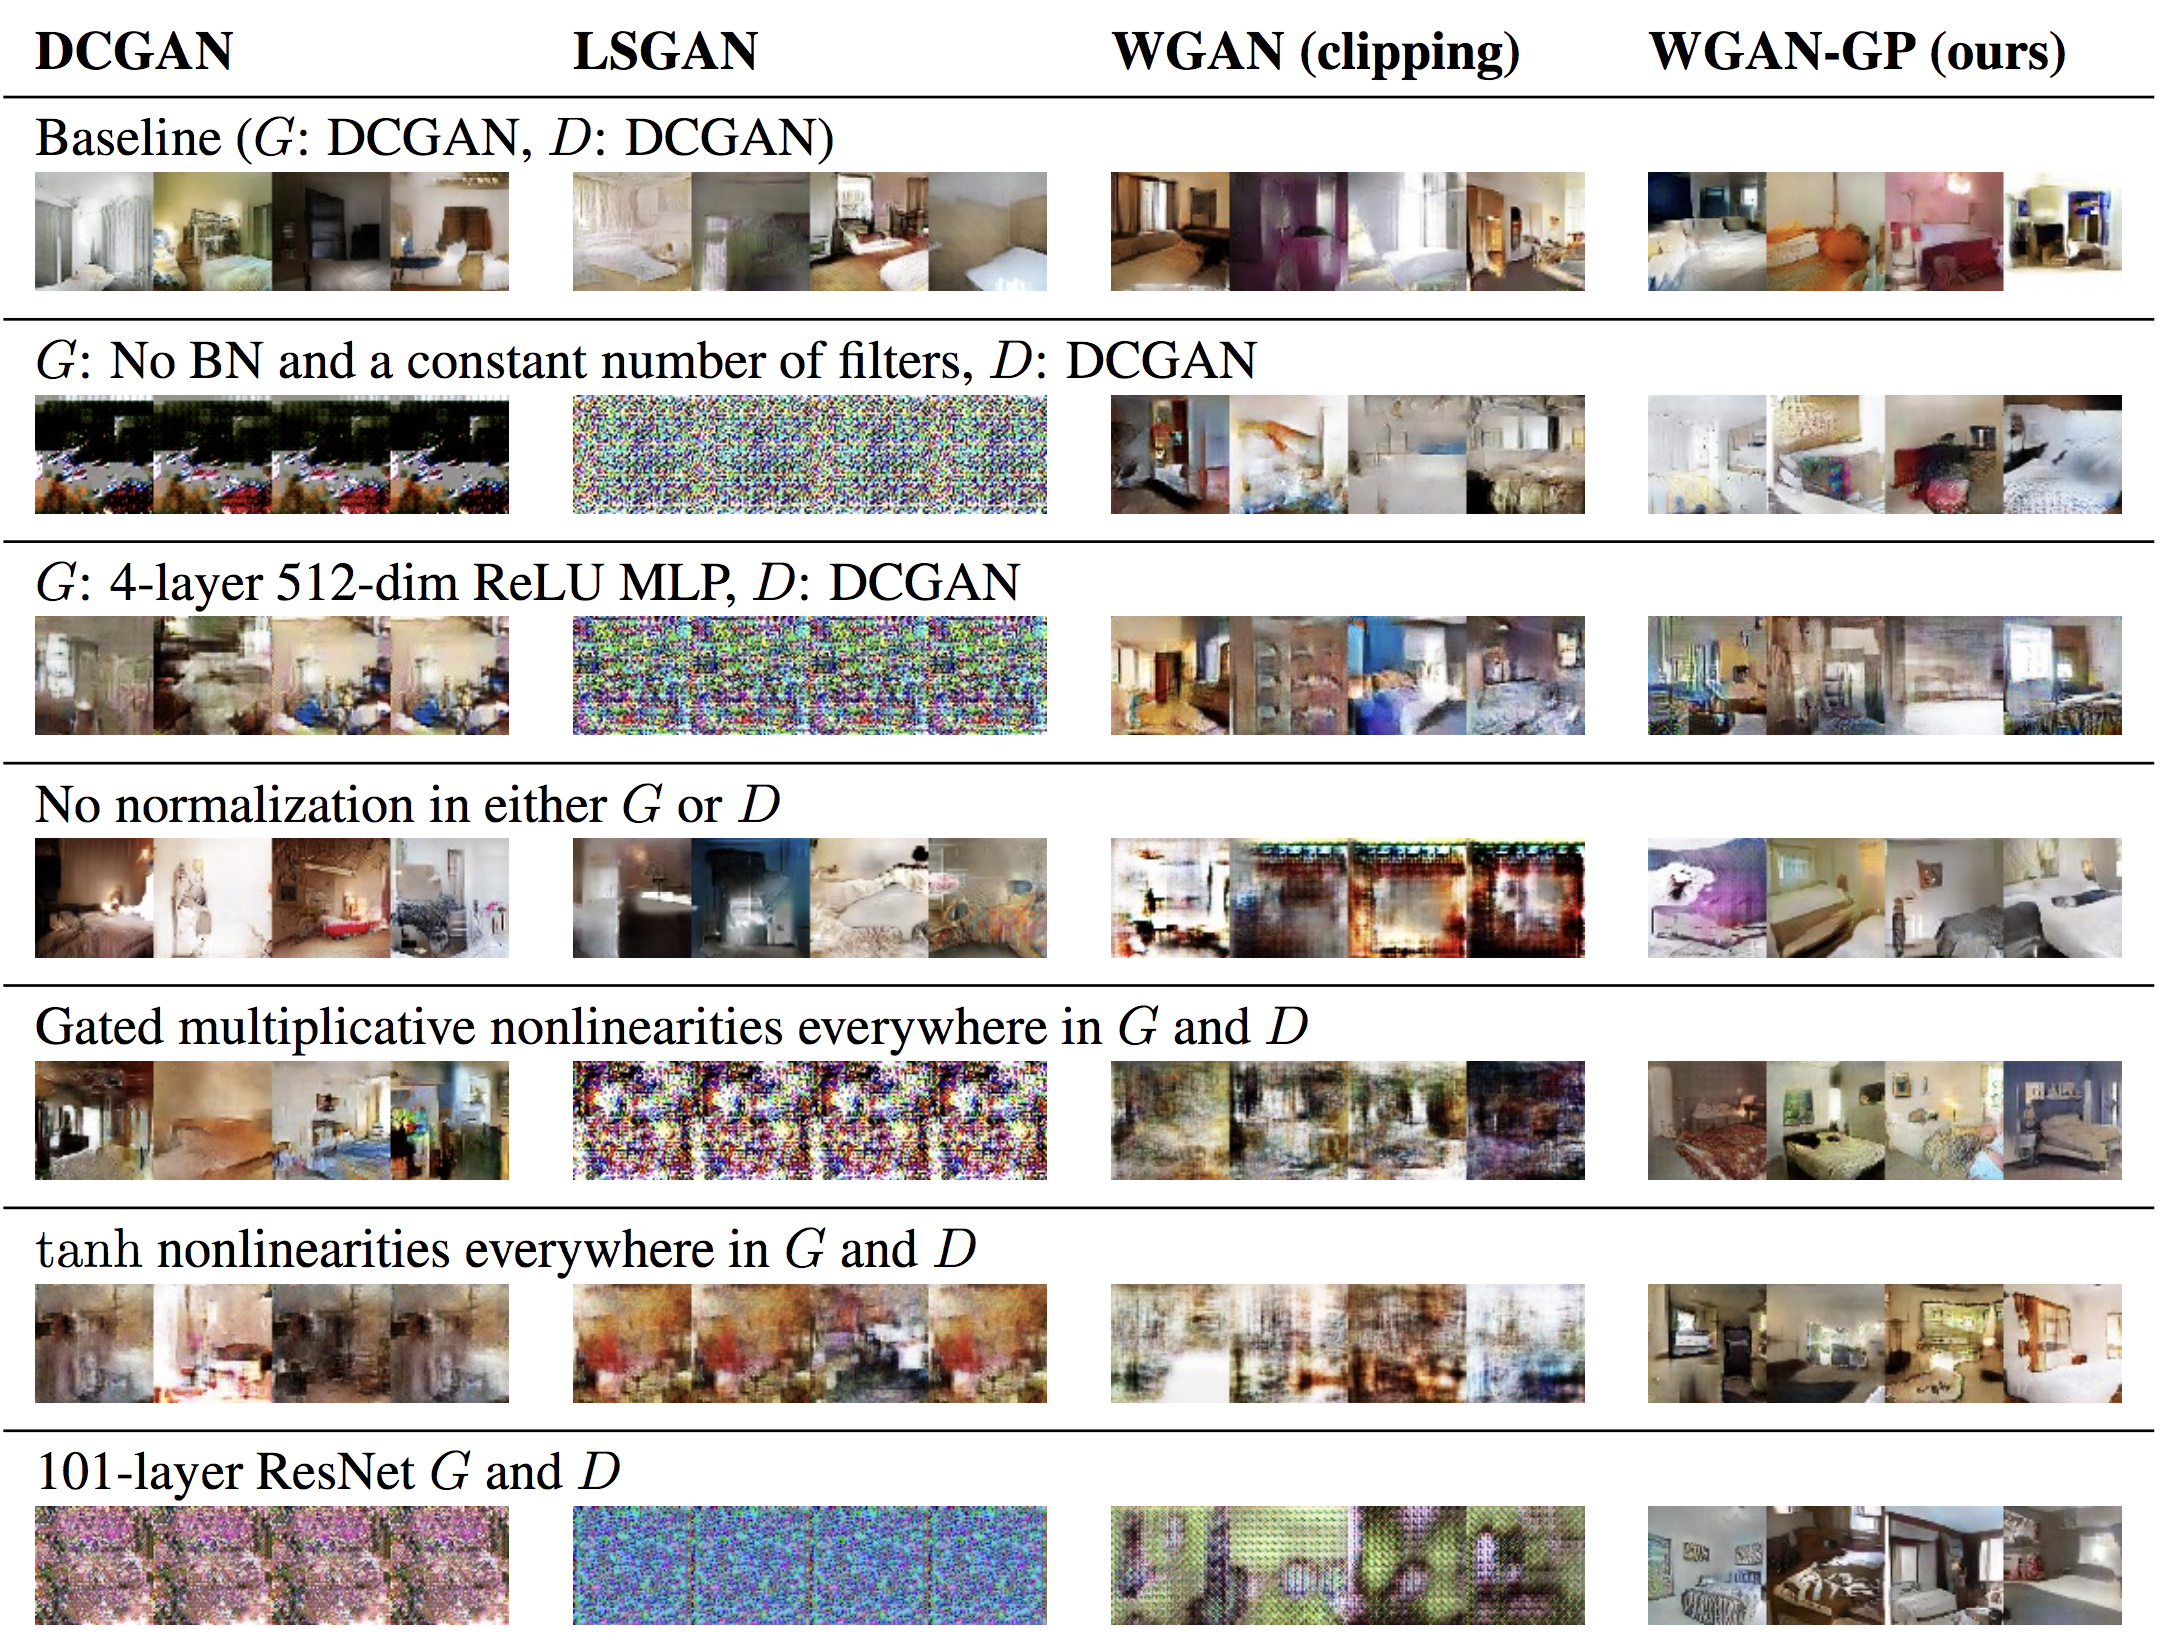
\includegraphics[height=0.85\textheight, width=1.05\textwidth, keepaspectratio]{images/gan/wgan-gp/slide_89_1_img.png}
        \caption*{[Gulrajani et al 2017]}
    \end{figure}
\end{frame}


\begin{frame}[allowframebreaks]{WGAN-GP: High quality samples}
    \begin{figure}
        \centering
        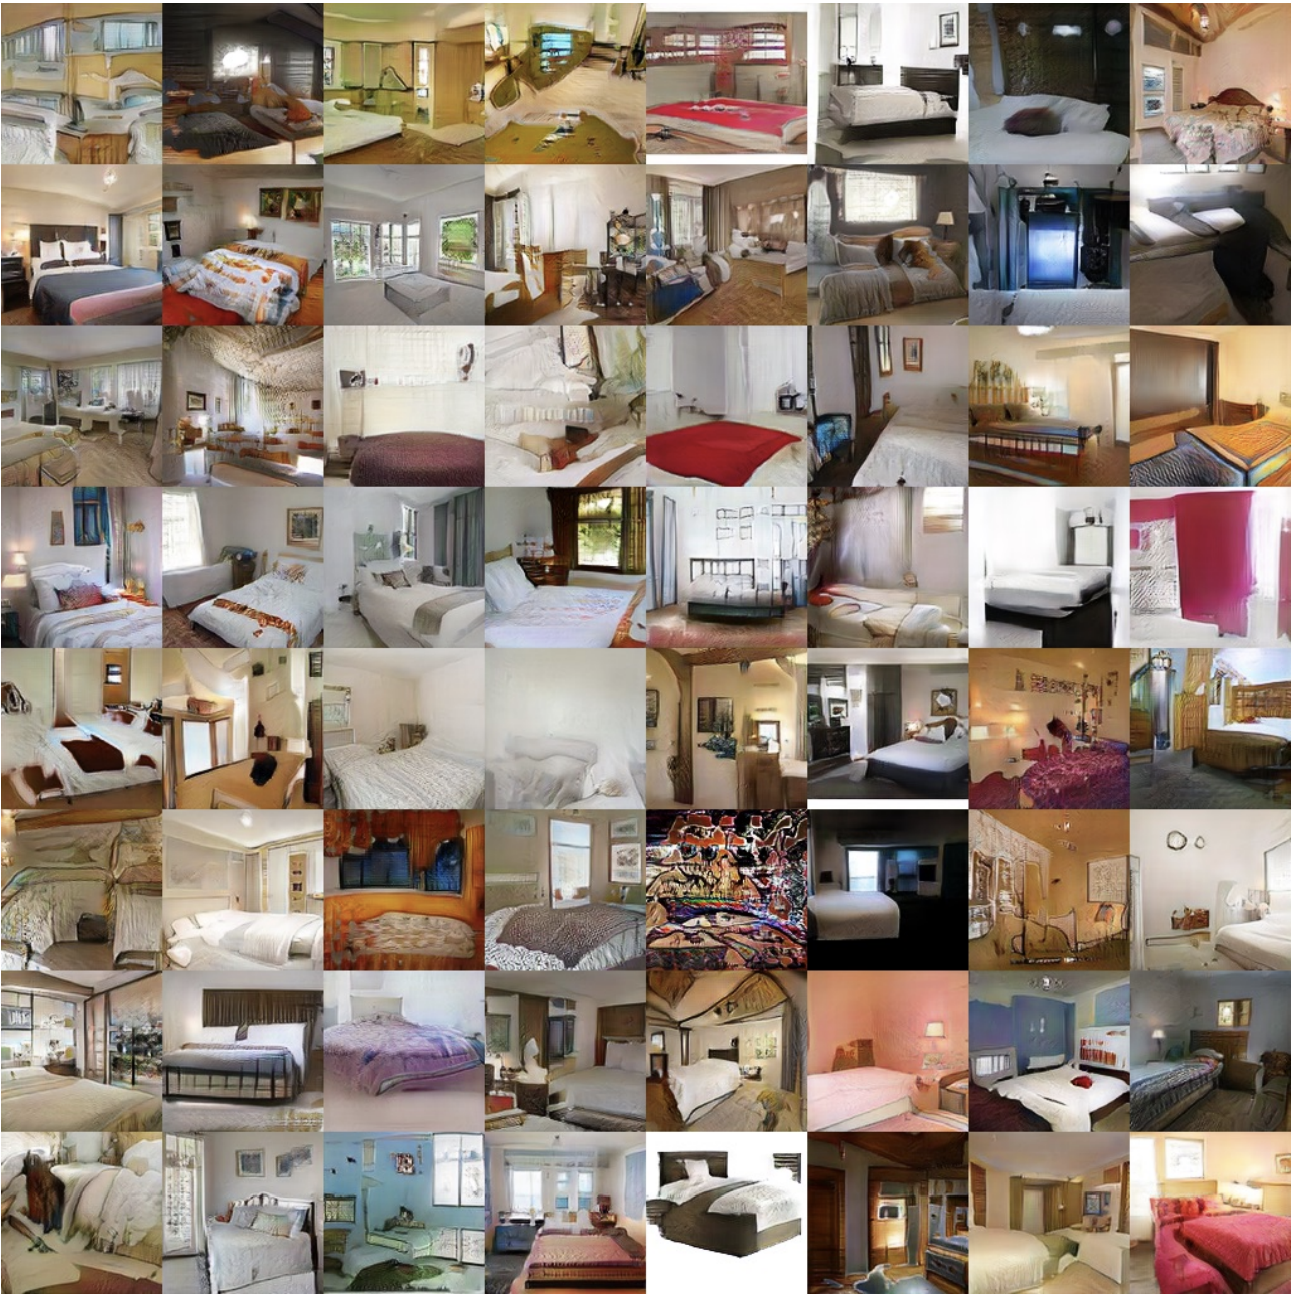
\includegraphics[height=0.8\textheight, width=1.05\textwidth, keepaspectratio]{images/gan/wgan-gp/slide_90_1_img.png}
        \caption*{[Gulrajani et al 2017]}
    \end{figure}

    \framebreak

    \begin{figure}
        \centering
        \includegraphics[height=0.8\textheight, width=1.05\textwidth, keepaspectratio]{images/gan/wgan-gp/slide_91_1_img.png}
        \caption*{[Gulrajani et al 2017]}
    \end{figure}
\end{frame}
\subsection{Conditional GANs}
\begin{frame}{}
    \LARGE GAN Variant: \\[1.5ex] \textbf{Conditional GANs}
\end{frame}

\begin{frame}[allowframebreaks]{Conditional GAN}
\begin{itemize}
    \item In addition to random noise, a condition is added to the generator input. 
    \item The discriminator also receives this condition.
\end{itemize}
\begin{figure}
    \centering
    \includegraphics[height=0.8\textheight, width=\textwidth, keepaspectratio]{images/gan/cond_gan_1.png}
\end{figure}

\framebreak
\begin{itemize}
    \item Discriminator Loss:
    \begin{align*}
    \mathcal{L}^{(D)} \left( \theta^{(G)}, \theta^{(D)} \right) =\ & 
    - \mathbb{E}_{x \sim p_{data}} \left[ \log D(x|y) \right] \\
    & - \mathbb{E}_{z \sim p_z(z),\ y \sim p_{data}(y)} \left[ \log(1 - D(G(z|y))) \right]
    \end{align*}
    \item Generator Loss:
    $$
    \mathcal{L}^{(G)} \left( \theta^{(G)}, \theta^{(D)} \right) = - \mathbb{E}_z \left[ \log D(G(z|y)) \right]
    $$
\end{itemize}

\framebreak
\begin{figure}
    \centering
    \includegraphics[height=0.8\textheight, width=\textwidth, keepaspectratio]{images/gan/cond_gan_2.png}
    \caption*{A conditional GAN architecture for the MNIST digits dataset.}
\end{figure}

\end{frame}

\begin{frame}[allowframebreaks]{Condional GAN - Image to Image}

\begin{figure}
    \centering
    \includegraphics[height=0.75\textheight, width=\textwidth, keepaspectratio]{images/gan/cond_gan_3.png}
    \caption*{Using L1 loss in addition in GAN loss can help in image to image translation}
\end{figure}

\framebreak

\begin{figure}
    \centering
    \includegraphics[height=0.8\textheight, width=\textwidth, keepaspectratio]{images/gan/cond_gan_4.png}
    \caption*{Image to Image translation with condional GANs}
\end{figure}
    
\end{frame}
\subsection{Cycle GANs}
\begin{frame}{}
    \LARGE GAN Variant: \\[1.5ex] \textbf{Cycle GANs}
\end{frame}


\begin{frame}[allowframebreaks]{Cycle GANs}

\begin{itemize}
    \item Unpaired Image-to-Image Translation using Cycle-Consistent Adversarial Networks, Efros, ICC7 2017
    
\end{itemize}
\begin{figure}
    \centering
    \includegraphics[height=0.7\textheight, width=\textwidth, keepaspectratio]{images/gan/cycle_gan_1.png}
\end{figure}
\framebreak
\textbf{Cycle Consistency}

\begin{itemize}
    \item \textbf{Cycle Consistency Loss:} Ensures that translating an image to the target domain and back yields the original image.
    \item For $x \in X$: $x \rightarrow G(x) = y \rightarrow F(y) \approx x$
    \item \textbf{Mathematically:}
    \[
        \mathcal{L}_{cyc}(G, F) = \mathbb{E}_{x \sim p_{data}(x)} \left[ \| F(G(x)) - x \|_1 \right] + \mathbb{E}_{y \sim p_{data}(y)} \left[ \| G(F(y)) - y \|_1 \right]
    \]
\end{itemize}

\framebreak
\textbf{Total Loss}

\begin{itemize}
    \item \textbf{Adversarial Loss:} Makes generated images indistinguishable from real images.
    \item \textbf{Cycle Consistency Loss:} Enforces reversibility of translation.
    \item \textbf{(Optional) Identity Loss:} Preserves color or structure.
    \item \textbf{Total Loss:}
    \[
        \mathcal{L}_{total} = \mathcal{L}_{GAN}(G, D_Y, X, Y) + \mathcal{L}_{GAN}(F, D_X, Y, X) + \lambda \mathcal{L}_{cyc}(G, F) + \gamma \mathcal{L}_{identity}
    \]
\end{itemize}
\framebreak
$$C_{horse \rightarrow zebra} = horse \rightarrow G_{horse \rightarrow zebra} \rightarrow \hat{zebra} \rightarrow [D_{zebra}, G_{zebra \rightarrow horse}] \rightarrow \hat{horse}$$
\begin{figure}
    \centering
    \includegraphics[height=0.7\textheight, width=\textwidth, keepaspectratio]{images/gan/cycle_gan_2.png}
\end{figure}

\framebreak
$$C_{zebra \rightarrow horse} = zebra \rightarrow G_{zebra \rightarrow horse} \rightarrow \hat{horse} \rightarrow [D_{horse}, G_{horse \rightarrow zebra}] \rightarrow \hat{zebra}$$
\begin{figure}
    \centering
    \includegraphics[height=0.7\textheight, width=\textwidth, keepaspectratio]{images/gan/cycle_gan_3.png}
\end{figure}

\framebreak
\begin{figure}
    \centering
    \includegraphics[height=0.7\textheight, width=\textwidth, keepaspectratio]{images/gan/cycle_gan_3.png}
\end{figure}

\framebreak
\begin{figure}
    \centering
    \includegraphics[height=0.9\textheight, width=\textwidth, keepaspectratio]{images/gan/cycle_gan_4.png}
\end{figure}

\framebreak
\begin{figure}
    \centering
    \includegraphics[height=0.9\textheight, width=\textwidth, keepaspectratio]{images/gan/cycle_gan_5.png}
\end{figure}

\framebreak
\begin{figure}
    \centering
    \includegraphics[height=0.9\textheight, width=\textwidth, keepaspectratio]{images/gan/cycle_gan_6.png}
    \caption*{Image to Image translation with Cycle GANs}
\end{figure}
\end{frame}
\subsection{Style GANs}
\begin{frame}{}
    \LARGE GAN Variant: \\[1.5ex] \textbf{Style GANs}
\end{frame}

\begin{frame}[allowframebreaks]{Style GANs}
\begin{itemize}
    \item Goal: Better disentanglement of features in latent space (\textbf{W} space)
\end{itemize}
    \begin{figure}
    \centering
    \includegraphics[height=0.9\textheight, width=\textwidth, keepaspectratio]{images/gan/stylegan_2.png}
\end{figure}

\footnotetext{https://www.cs.unc.edu/~ronisen/teaching/fall_2022/pdf_lectures/lecture6_gan2.pdf}
\end{frame}
\begin{frame}[allowframebreaks]{Style GANs}
\begin{figure}
    \centering
    \includegraphics[height=0.9\textheight, width=\textwidth, keepaspectratio]{images/gan/stylegan_1.png}
\end{figure}
\footnotetext{https://arxiv.org/pdf/1812.04948}
\end{frame}
\begin{frame}[allowframebreaks]{Style GANs}

\begin{itemize}
    \item \textbf{A} = learned affine transformation block for AdaIN (predicts y)
    \item \textbf{Ada}ptive \textbf{I}stance \textbf{N}ormalization (very effective in controlling styles)
    $$\text{AdaIN}(x_i,y) = y_{s,i}\frac{x_i - u(x_i}{\sigma(x_i)} + y_{b,i}$$
    \item \textbf{B} = learned per-channel scaling factor for noise input.

\end{itemize}

\end{frame}

\begin{frame}[allowframebreaks]{Which Latent space to choose for embedding and editing?}
\begin{itemize}
    \item \textbf{Z} : 512 dimensional latent space (not good)
    \item \textbf{W} : 512 dimensional latent space (better but not perfect)
    \item \textbf{W+} : 18x512 dimensional latent space (after affine transformation \textbf{A} has been applied)
    \item \textbf{W} is better for editing.
    \item \textbf{W+} is better for reconstruction or embedding of real images.
\end{itemize}

\end{frame}

\begin{frame}[allowframebreaks]{Style GANs - Results}
\begin{figure}
    \centering
    \includegraphics[height=0.9\textheight, width=\textwidth, keepaspectratio]{images/gan/stylegan_3.png}
\end{figure}
\footnotetext{https://arxiv.org/pdf/1812.04948}
\end{frame}
\section{Latent space Interpolation}
\begin{frame}{}
    \LARGE GANs: \textbf{Latent space Interpolation}
\end{frame}

\begin{frame}[allowframebreaks]{Latent space Interpolation}
\begin{figure}
    \centering
    \includegraphics[height=0.9\textheight, width=\textwidth, keepaspectratio]{images/gan/gan_latent.png}
    \caption*{Latent space interploation with GANs}
\end{figure}
\framebreak
\centering
Latent space interpolation with StyleGAN\\
\centering
(Demo by Xander Steenburgge)\\

\vspace{\baselineskip}

\centering
\href{https://colab.research.google.com/drive/1mH70YxGNlnEaSOn0J8Lsgkl-QOvsIb3M#scrollTo=uEhxBvAR-7y3}{https://colab.research.google.com/drive/1mH70YxGNlnEaSOn0J8Lsgkl-QOvsIb3M#scrollTo=uEhxBvAR-7y3}
\end{frame}
\section{More Results}
\begin{frame}{}
    \LARGE GANs: \textbf{More Results}
\end{frame}

\begin{frame}[allowframebreaks]{Some more GAN results}
\begin{figure}
    \centering
    \includegraphics[height=0.8\textheight, width=\textwidth, keepaspectratio]{images/gan/gan_results_4.png}
    \caption*{Image Inpainting. https://www.nvidia.com/en-us/research/ai-demos/}
\end{figure}

\framebreak

\begin{figure}
    \centering
    \includegraphics[height=0.8\textheight, width=\textwidth, keepaspectratio]{images/gan/gan_results_5.png}
    \caption*{Text to Image Synthesis with GANs}
\end{figure}

\framebreak

\begin{figure}
    \centering
    \includegraphics[height=0.8\textheight, width=\textwidth, keepaspectratio]{images/gan/gan_results_6.png}
    \caption*{Living Portraits with GANs}
\end{figure}

\begin{figure}
    \centering
    \includegraphics[height=0.8\textheight, width=\textwidth, keepaspectratio]{images/gan/gan_results_7.png}
    \caption*{Image to Image translation in multiple domains with StyleGAN (Choi et al.)}
\end{figure}
\end{frame}
\begin{frame}[allowframebreaks]{Autoregressive Models: Summary}
    \begin{itemize}
        \item Define a specific order for the variables in the data (e.g., $x_1, x_2, \ldots, x_n$).
        \item Model the joint probability as a product of conditional probabilities: 
        \[
            \mathcal{P}(X = \overline{x}) = \prod_{i=1}^n \mathcal{P}(x_i \mid x_{<i})
        \]
        \item Sampling is performed recursively: generate $x_1$ first, then $x_2$ conditioned on $x_1$, and so on.
        \item Efficient to compute likelihoods and log-likelihoods for both discrete and continuous variables.
        \item Flexible: can be extended to multi-class, multi-dimensional, and structured data.
        \framebreak
        \item Limitations:
        \begin{itemize}
            \item No natural way to extract global features or representations.
            \item Not inherently suited for clustering or unsupervised learning tasks.
            \item The choice of variable ordering can significantly affect performance.
        \end{itemize}
    \end{itemize}
\end{frame}

\begin{frame}{References}
Reference Slides
\begin{itemize}
    \item Fei-Fei Li "Generative Deep Learning" CS231
    \item Hao Dong "Deep Generative Models"
\end{itemize}
    
\end{frame}
\section{Limitations of Transformers}
\begin{frame}
    \frametitle{Limitations of Transformers}
    \begin{itemize}
        \item High compute and memory requirements
        \item Poor extrapolation capabilities
        \item Limitations due to hard-coded positional encoding
        \item Quadratic attention cost ($O(n^2)$)
        \item Lack of reasoning and grounding
    \end{itemize}
\end{frame}

\section{Future Directions}
\begin{frame}
    \frametitle{Future Directions}
    \begin{itemize}
        \item Linear and sparse attention mechanisms
        \item Memory-efficient transformers (e.g., FlashAttention)
        \item Integration with retrieval, reasoning, and tool use
        \item Multimodal transformers (e.g., Flamingo, GPT-4V)
        \item Biologically inspired architectures (e.g., RWKV, State Space Models)
    \end{itemize}
\end{frame}
\begin{frame}{}
    \LARGE Generative AI for Science: \textbf{References}
\end{frame}

\begin{frame}[allowframebreaks]{References}
    \begin{itemize}
        \item AlphaFold: Jumper, J., Evans, R., Pritzel, A., Green, T., Figurnov, M., Ronneberger, O., ... \& Hassabis, D. (2021). Highly accurate protein structure prediction with AlphaFold. Nature, 596(7873), 583-589.
        \item Earth-2: NVIDIA. (2022). Earth-2: A Digital Twin of the Earth for Climate Research. Retrieved from \url{https://www.nvidia.com/en-us/research/earth-2/}
        \item SMILES: Weininger, D. (1988). SMILES, a chemical language and information system. 1. Introduction to methodology and encoding rules. Journal of Chemical Information and Computer Sciences, 28(1), 31-36.
    \end{itemize}
    \framebreak
    \begin{itemize}
        \item FourCastNet: Salazar, J., & Koster, R. D. (2021). FourCastNet: A global data-driven high-resolution weather model. Nature, 591(7849), 234-239.
        \item ChemDFM: Zhang, Y., Wang, H., & Liu, B. (2023). ChemDFM: A foundation model for chemistry. Cell, 186(1), 1-15.
        \item Science Advances: Chen, H., & Zhang, Y. (2023). Leveraging negative reactions for improved reactivity predictions. Science Advances, 9(12), eadk1426.
    \end{itemize}
    \framebreak
    \textbf{Additional Resources:}
    \begin{itemize}
        \item NVIDIA Earth-2: \url{https://build.nvidia.com/nvidia/fourcastnet?snippet_tab=Try}
        \item SMILES: \url{https://www.daylight.com/dayhtml/doc/theory/theory.smiles.html}
        \item AlphaFold: \url{https://alphafold.ebi.ac.uk/}
        \item Earth-2: \url{https://www.nvidia.com/en-us/research/earth-2/}
    \end{itemize}
\end{frame}
\begin{frame}[allowframebreaks]{Appendix: Additional Resources}
\large
\textbf{Learning: Estimate frequencies by counting}
\normalsize
\begin{columns}
    \begin{column}{0.55\textwidth}
       \begin{itemize}
            \setlength{\itemsep}{0.75em}
            \item Recall: the goal is to estimate $p_{\text{data}}$ from samples $x^{(1)}, \ldots, x^{(n)} \sim p_{\text{data}}(x)$
            \item Suppose the samples take on values in a finite set $\{1, \ldots, k\}$
            \item The model: a histogram
            \begin{itemize}
                \item (Redundantly) described by $k$ nonnegative numbers: $p_1, \ldots, p_k$
            \end{itemize}
            \item To train this model: count frequencies
            \item $p_i = \frac{\# \text{ times } i \text{ appears in the dataset}}{\# \text{ points in the dataset}}$
        \end{itemize}
    \end{column}
    \begin{column}{0.45\textwidth}
        \begin{figure}
            \centering
            \includegraphics[width=1.1\textwidth,keepaspectratio]{images/arm/histogram_training.png}
        \end{figure}
    \end{column}
\end{columns}

\framebreak

\large
\textbf{Inference and Sampling}
\normalsize
\begin{itemize}
    \setlength{\itemsep}{0.75em}
    \item \textbf{Inference (querying $p_i$ for arbitrary $i$):} simply a lookup into the array $p_1, \ldots, p_k$
    \item \textbf{Sampling (lookup into the inverse cumulative distribution function):}
    \begin{itemize}
        \item From the model probabilities $p_1, \ldots, p_k$, compute the cumulative distribution:
        \[
            F_i = p_1 + \cdots + p_i \quad \text{for all } i \in \{1, \ldots, k\}
        \]
        \item Draw a uniform random number $u \sim [0, 1]$
        \item Return the smallest $i$ such that $u \leq F_i$
    \end{itemize}
    \item \textbf{Are we done?}
\end{itemize}

\framebreak

\large
\textbf{Problem: Lack of Generalization}
\normalsize
\begin{columns}
    \begin{column}{0.45\textwidth}
        \begin{figure}
            \centering
            \includegraphics[width=\textwidth,keepaspectratio]{images/arm/histogram_training.png}
        \end{figure}
        \begin{figure}
            \centering
            \includegraphics[width=\textwidth,keepaspectratio]{images/arm/histogram_test.png}
        \end{figure}
    \end{column}
    \begin{column}{0.55\textwidth}
       learned histogram = training data distribution 

        → often poor generalization
    \end{column}
\end{columns}

\framebreak

\large
\textbf{Solution: Parameterized Distributions}
\normalsize
\begin{columns}
    \begin{column}{0.45\textwidth}
        \begin{figure}
            \centering
            \includegraphics[width=\textwidth,keepaspectratio]{images/arm/histogram_training.png}
        \end{figure}
        \begin{figure}
            \centering
            \includegraphics[width=\textwidth,keepaspectratio]{images/arm/histogram_test.png}
        \end{figure}
    \end{column}
    \begin{column}{0.55\textwidth}
       \begin{figure}
            \centering
            \includegraphics[width=\textwidth,keepaspectratio]{images/arm/histogram_parameterised.png}
            \caption{Fitting a parameterized distribution often generalizes better than a histogram.}
        \end{figure}
    \end{column}
\end{columns}
    
\end{frame}


\input{sections/credits}

\end{document} 